\documentclass[10pt,conference,compsocconf]{IEEEtran}

\usepackage{hyperref}
\usepackage{graphicx}	% For figure environment
\usepackage{mathptmx}
\usepackage{helvet}
\usepackage{courier}
\usepackage{graphicx}
\usepackage{imakeidx} \makeindex[options = -s svind]
\usepackage{multicol}
\usepackage[bottom]{footmisc}
\usepackage{natbib}
\bibliographystyle{humannat}
\usepackage{amssymb}
\usepackage{amsmath}
\usepackage{float}
%\restylefloat{table}
%\usepackage{floatrow}
%\floatsetup[table]{capposition=top}
%\usepackage{lscape}
\usepackage{breqn}
%\usepackage{listings}
\usepackage{color}
%\usepackage[utf8]{inputenc}
%\usepackage{array}
%\definecolor{mygreen}{RGB}{28,172,0}
%\definecolor{mylilas}{RGB}{170,55,241}
\def\one{\mbox{1\hspace{-4.25pt}\fontsize{12}{14.4}\selectfont\textrm{1}}}
\newcommand{\plim}{\text{plim}}
\newcommand{\tr}{\text{tr}}
\newcommand{\diag}{\text{diag}}
\newcommand{\rank}{\text{rank}}
\newcommand{\Exp}{\text{E}}
\newcommand{\vect}{\text{vec}}
\newcommand{\vech}{\text{vech}}
\newcommand{\Var}{\text{Var}}
\newcommand{\lnf}{\text{ln f}}
\newtheorem{assumption}{Assumption}
\usepackage{amsmath}
\usepackage{breqn}
\newcommand{\R}{\mathbb{R}}

\begin{document}
\title{Project 2}

\author{
Bilguun Chinzorig, Monika Avila, Lkham Nyambuu\\
  \textit{EPFL}
}

\maketitle

\begin{abstract}
  The aim of this project is to conduct a twitter sentiment analysis. Our goal is to classify untaged tweets into two groups: positive and negative. 
  For this purpose, we begin our work by preprocessing the tweets and generate the dictiorany. Following, we create the word space, i.e. matrix of embeddings using GloVe methodology. After, we span the tweet space by retrieving features from the embedding matrix. In addition to these features, we constructed additional variables that capture the meaning  and the importance of the words as well as hashtags included in each tweet. Finally, we used our futures in two types of classifiers: 1. Random Forests and 2. SVM. 
  We conclude that random forests outperforms SVM considering both computing efficiency and classifying results. 
\end{abstract}	\textbf{ }

\section{Introduction}



\section{The vocabulary construction: Word preprosecing}

We begin our work by preprocessing the available tweets such that we can define our vocabulary. However the words in the dataset are not easily separable by whitespaces due to following reasons:
	
	\textbf{Separators:} Words can be separated by multiple characters including whitespace for words, period for sentence ending, comma for clause endings, dash for connected words and : or ; to for beginning independent clauses. The problem is that the last two characters can be used as emojis. 

\textbf{Word contractions:} word contractions can be viewed as complete new token, but in the end it is just combination of two words. Common word contractions are related to to be's and modal verbs.

\textbf{Special words:} Due to freedom of writing tweets, we can observe multiple emphasizes on words including hashtags, and repeated characters like (hey to heyyyy). These words must have a special treatment but for vocabulary building these variations were eliminated.

\textbf{Stop words:} The full list of stop words can be found here https://kb.yoast.com/kb/list-stop-words/. In our case, we are assuming pronouns like "the" can represent some meaningful information since it emphasizes following nouns.

\textbf{Word variations:} In english word can take multiple forms like plural form, verb tenses, incorrect spelling etc. Hence, simple word separation is not enough. And also in english, people use "'s" or "s'" to represent possessions REPHRASE THIS!! 

\textbf{Numbers:} we assumed that numbers usually conveys factual informations which is not helpful to identify the opinion of a person. Moreover, we need to treat numbers different from words. Thus, we have completely removed every numbers.

In order to overcome the problems mentioned above, we created a customized vocabulary building algorithm with the following procedure:

First we tokenized the text using white space, comma, period, new line. We excluded : and ; since they are maybe part of emojis.
Following, for each token we look for word contractions. In our case, we only considered hashtags, common contraction list to separate tokens which contains multiple words. Moreover, we have removed possessions from each token.
After this, we address the issue of word variation by shrinking consecutive repeated characters, e.g. we replaced "fooooot" by "foot". Finally, we used their stems to build our vocabuary.

This preprocesing lead to an increase of the tokens in 80,000. Moreover, the total number of unique words in decreased significantly. Indeed, we have successfully obtained almost 32,000 unique words. This means that we ended up with just 32\% of all the tokens produced after splitting. (Clarify)

Now let's look at the distribution of each words. The graph \ref{fig1} shows the distribution of the words of our final vocabulary. As expected, it shows similar relationship as Zipf's law, but note that the number of words with only 1 occurence in the entire text is important. Indeed, almost 50\% of the vocabulary takes only 1.2\% of the text which implies that it is not worth keeping the 50\% of the words for simplicity.

Finally, in order to increase efficiency of the information contained in our final co-ocurence matrix we apply term frequency- inverse document frequency (tf-idf) feature. This factor gives more importance to words that are repeated in a tweet but not highly recurrent in the whole corpora.  

\begin{tiny}
		\begin{figure}[b] \label{fig1}
			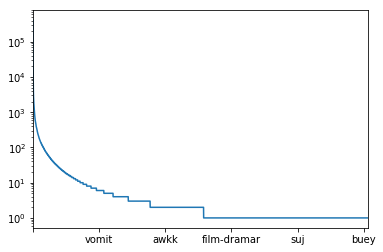
\includegraphics[scale=0.5]{WordDistribution.png}   
			\caption{Word Distribution }
			\label{fig1}    
		\end{figure}
\end{tiny}

\section{The word space: embedding matrix }
\label{S1}
In order to obtain a numerical representation of the words $w_i$ contained in the data set  as $\textbf{w}_{\textbf{i}} \in \mathbb{R}^K$ we used GloVE model. 

This model retrieves the numerical representation of the words that is closest to natural logarithm of the observed co-occurence value $x_{ij}$. Indeed,  \cite{pennington2014glove} propose to obtain the real valued vector by minimizing a weighted sum of squared errors. Where the error is the difference between the log of co-occurence value and the predicted one given by $\textbf{w}'_{\textbf{i}}\textbf{w}_{\textbf{j}}$. Thus, the model minimizes the following cost function: 

$$L(\textbf{w}_{\textbf{n}},\textbf{w}_{\textbf{c}})=\sum_{j=1}^{N}\sum_{i=1}^{D}f(x_{ij})(log(x_{ij})-\textbf{w}'_{\textbf{i}}\textbf{w}_{\textbf{j}})^2$$ 

with: 
$$f(x_{ij})=min(1,x_{ij}/x_{max})^{3/4}$$ 
\section{The tweet space: feature retrieval}
In order to obtain a numerical representation of the tweet space we retrieved two types of features. The first class is obtained using GloVe matrix of embeddings. On contrast, we developed the second type of features with the aim to capture the syntax.

Using the GloVe matrix of embeddings, we used the mean of the word embedings. 

On the other hand, the features that we developed are: 

\begin{enumerate}
	\item The mean of the tf-idf. 
	\item The weighted sum of the tf-idf, which means that we weighted hashtaged  tf-idf, positive tags  tf-idf, negative tags  tf-idf and emphasis  tf-idf.  		
	\end{enumerate}

\section{The Classification Model}
After obtaining the tweet space i.e. the features that represent the data set of tweets, we trained the classification model. For this aim, we used two models: 1. Random Forest and 2. SVM. 

The first model is random forests, this is a method based in an ensemble approach composed of a set of decision trees. At each node, the variables used to divide the space of the independent variables are randomly selected and used to create the decision tree (\cite{breiman2001random}). 

The second classification algorithm used is SVM. In this method, we look to maximize the geometric margin between positive and negative tweets subject to the constraint that the classified vectors must lie outside this margin\footnote{AndrewNg, Support Vector Machines}. This optimization problem is equivalent to the following one for each training sample:

$$min_w || w ||^2$$
$$s.t. \quad y_i(x'_iw +b)\geq 1$$

 Now, setting the dual problem we can obtain the support vectors which are few training observations that lie on the margin. 
 
%\section{Methods}
%\label{S2}



\section{The Data}
\label{S3}

The training data set is formed by 2 millions of tweets, half of them correspond to the positive emotions and the other half to negative ones. This data has been already tokenized, thus we start with the cleaning and the analysis of the data.  

%First, we remove the hashtags, URL directions and @... 

%Second, we  counting the words and we check Zipf's law.


\section{Results}
\label{S4}

\section{Discussion}
\label{S5}

\section{Summary}
\label{S6}

\bibliography{Project2}
\bibliographystyle{spbasic}
\end{document}